\documentclass[12pt, a4paper]{article}
\usepackage[utf8]{inputenc} 
\usepackage[margin=1.2in]{geometry}
\usepackage{multicol}
\usepackage{multirow}
\usepackage{url}
\usepackage{graphicx}
\usepackage{amsfonts}
\usepackage[tbtags]{amsmath}
\usepackage{amsmath}
\usepackage{caption}
\usepackage{subcaption}
\usepackage{float}
\usepackage{pdfpages}

\title{
	\line(1,0){300}
	\endgraf\bigskip
	\Huge
	\begin{center}
		\emph{CC-AODV: An Effective Multiple Paths Congestion Control AODV} 
		%\emph{\Large{}}
		
	\end{center}
	\line(1,0){300}
	\bigskip
	\bigskip
}

\author{
    \large{Kawshik Kumar Paul}\\
	\large{Student ID : 1705043}\\
	\large{Undergrad Student}\\\\\\
	\Large{Department of Computer Science and Engineering}\\
    \Large{Bangladesh University of Engineering and Technology}\\\\\\\\\\
}

\date{
	\endgraf\bigskip
	\Large{\today}
}
\begin{document}
\maketitle
\pagebreak
\tableofcontents
\pagebreak
\section{Network Topologies Under Simulation}
\subsection{Topology for Task A - Wired}
A wired topology is used which is look alike Fig \ref{fig:task_a_wired} which is built with two LAN networks and a Point to Point network connecting the two LANs.\\
Packet is sent from one LAN network to another LAN network in simulation.
\begin{figure}[H]
\centering
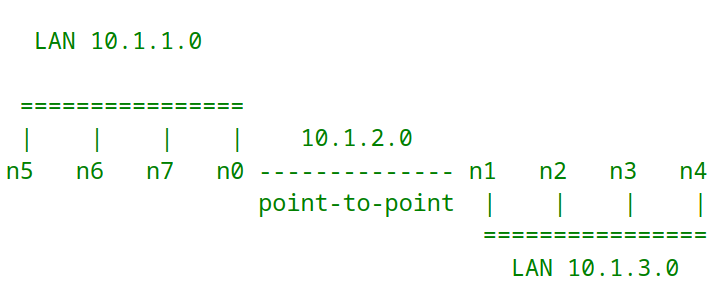
\includegraphics[scale = 0.6]{images/wired-01.png}
\caption{Wired Topology}.
\label{fig:task_a_wired}
\end{figure}

\subsection{Topology for Task A - Wireless Low Rate (Static)}
IEEE standard 802.15.4 intends to offer the fundamental lower network layers of a type of wireless personal area network (WPAN) which focuses on low-cost, low-speed ubiquitous communication between devices.
Here in this simulation, low rate wpan devices (lrwpan devices) are used.
\begin{figure}[H]
\centering
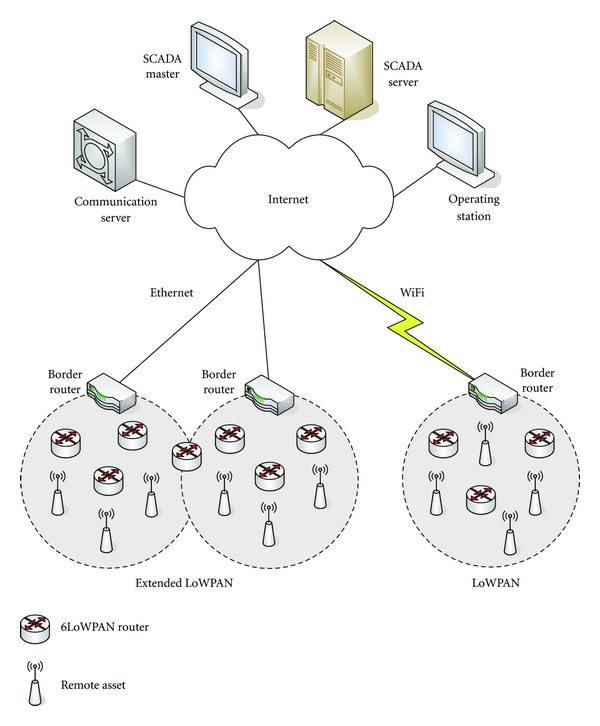
\includegraphics[scale = 1]{images/6LoWPAN.png}
\caption{Wireless Low Rate Network Topology}.
\label{fig:task_a_wired}
\end{figure}
\subsection{Topology for Task B - MANET AODV}
MANET is a dynamic wireless network that can be formed without the need for any pre-existing infrastructure. So, the network topology may be changed dynamically in an unpredictable manner since nodes are free to move.

\begin{figure}[H]
\centering
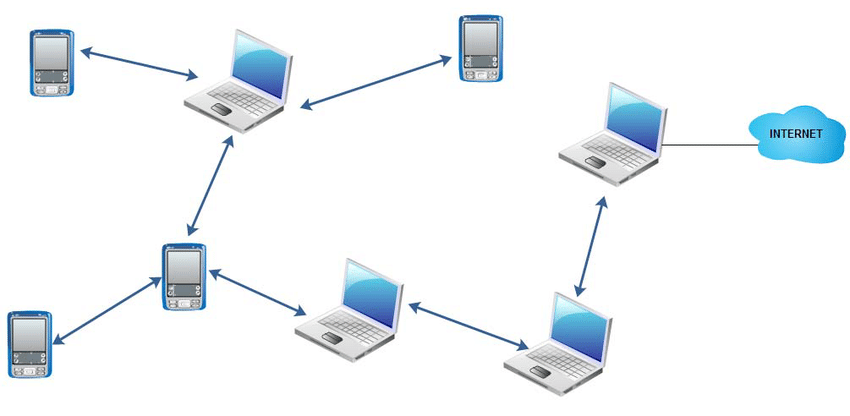
\includegraphics[scale = 0.6]{images/MANET.png}
\caption{Adhoc Network Topology}.
\label{fig:task_a_wired}
\end{figure}


\section{Parameters Under Variation}
\subsection{Parameters for Task A - Wired}

In this network topology, I had to simulate a wired topology.
I have varied the following parameters,
\begin{enumerate}
    \item The number of nodes varied as (20, 40, 60, 80, and 100)
    \item The number of flows (10, 20, 30, 40, and 50) 
    \item The number of packets per second (100, 200, 300, 400, and 500) 
\end{enumerate}
\subsection{Parameters for Task A - Wireless Low Rate (Static)}
In this network topology, I had to simulate a wireless low rate (802.15.4) static network. I have varied the following parameters.
\begin{enumerate}
    \item The number of nodes varied as (20, 40, 60, 80, and 100)
    \item The number of flows (10, 20, 30, 40, and 50) 
    \item The number of packets per second (100, 200, 300, 400, and 500)
    \item Coverage area (square coverage are varying one side as Tx\_range, 2 x Tx\_range, 3 x Tx\_range, 4 x Tx\_range, and 5 x Tx\_range)
\end{enumerate}
\subsection{Parameters for Task B - MANET AODV}
According to my selected paper, the number of nodes and sinks are varied to make the simulation.
\pagebreak

\section{ Overview of the Proposed Algorithm }
MANETs are characterized by wireless mobile
nodes in a network that supports the functionality of self-
configurable and independently movable nodes. These nodes in
turn can be shape as hosts or clients to construct dynamic
networks for package delivery from its source to their respective
destinations via dynamic routing path. Regarding the network
performance, routers perform a critical role of delivering the data
to the appropriate destinations. Engineers have been
implementing various routing algorithms to improve wireless
network performance. Ad hoc On-Demand Distance Vector
(AODV) routing is one of the famous routing algorithms.
Tremendous amounts of research on this protocol have been done
to improve the performance. In this paper, a new control scheme,
named congestion control AODV (CC-AODV), is proposed to
manage the described routing condition. With this table entry, the
package delivery rates are significantly increased while the
package drop rate is decreased, however its implementation causes
package overhead. This paper uses NS3 (network simulator 3) for
simulation.


\subsection{What is AODV?}
    An Ad Hoc On-Demand Distance Vector (AODV) is a routing protocol designed for wireless and mobile ad hoc networks. This protocol establishes routes to destinations on demand and supports both unicast and multicast routing.\\
    \subsubsection{Route Discovery}
    \begin{itemize}
        \item In AODV, the route is requested only when the source node
        wants to send data to the desired destination node. Hence, the
        source node starts to send RREQ to its neighboring nodes
        initiating communication.
        \item When an intermediate node received the RREQ packets, the
        routing table adds the routing information. If the table already
        has the entry, then the routers compare the sequence number
        and hop count with the existing information in the table. If the
        condition passes, the table will update the routing information
        in the table.
        \item After receiving RREQ, node determines whether it is the destination node or not. Moreover, the node can check whether it received the same RREQ packets with the same ID previously. As a result, if a node receives the same ID packets, then it determines whether it requires an update to the table or not.
        \item Once a destination node receives a RREQ packet, it
        generates the routing reply packets (RREP). This packet
        unicasts back to its represented source node and updates the
        intermediate node routing table. Thus, AODV establishes the
        routing path.
    \end{itemize}
    \subsubsection{Route Maintenance}
    \begin{itemize}
        \item Once a link has failed or the connection is lost, a router
        error (RRER) packet is generated and sent to the source node,
        which in turn requests to establish the new routing path.
        \item When the source node receives the RRER packets, it starts the flooding broadcast of RREQ packets to reinitiate the route
        again, allowing AODV to maintain the routing path.
    \end{itemize}
\subsection{Issues with AODV}
Though sometimes intermediate nodes are too busy to transmit data
packages, yet those nodes are used since they are on the shortest
path of communication. Nonetheless, when using this approach
other nodes that are available are not fully utilized even if they
might have low traffic, leading to a lack of bandwidth
utilization. As a result, the performance is degraded as the
delays in delivering packets increase as well as the number of
packets delivered is reduced.
\subsection{Proposed CC-AODV Mechanism}
To overcome the challenge of AODV, the congestion control CC-ADOV is proposed.
\begin{itemize}
    \item The proposed CC-ADOV aims to lower the performance
    degradation caused by the packets congestion while the data is
    delivered using AODV.
    \item CC-AODV determines a path for the data by using the congestion counter label. This is achieved by checking how stressed the current node is in a table, and once the RREP package is generated and transmitted through the nodes, the congestion counter adds one to the counter.
    \item The process of CC-AODV flow chart explains how to
establish the route in Fig \ref{fig:cc-aodv-algo}.
\end{itemize}
\subsubsection{Flowchart}
\begin{figure}[H]
\centering
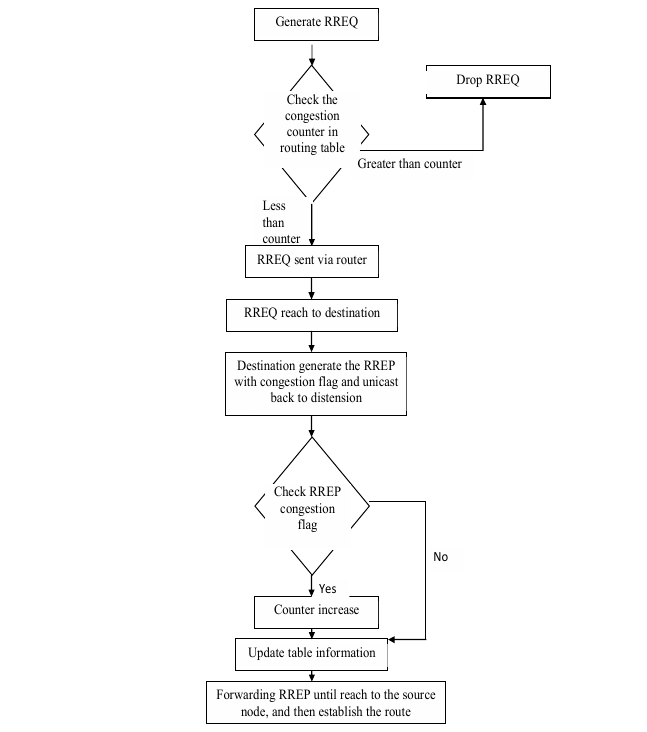
\includegraphics[scale = 0.6]{images/cc-aodv/cc-aodv-algo.png}
\caption{Process of CC-AODV flow chart}.
\label{fig:cc-aodv-algo}
\end{figure}
\subsubsection{Algorithm}
\begin{itemize}
    \item First, the source node performs a
    flooding broadcast RREQ package in the entire network.
    \item When RREQ package arrives to the intermediate node, the router checks the congestion counter whether it is less than a certain predetermined value.
    \item If the comparison yields less than the counter, the routing table updates and forwarding to next router; otherwise, the router drops the RREQ package.
    \item Once the RREQ arrives to the corresponding destination, the RREP is generated by the router. In CC-AODV, the congestion flag is added to the RREP header.
    \item  There are two cases of which a RREP is generated corresponding to a RREQ. One is from the source node to establish the route and the other is from the neighbor nodes to maintain the route.
    \item When the destination node receives the RREQ from the source node, it generates the RREP with the congestion flag set to true. While the RREP unicast back to the corresponding source node, passing by the intermediate node, the router checks the congestion flag. If it is true, the counter increases; otherwise, the counter keeps the same. Then, the router updates the routing information.

\end{itemize}
\subsubsection{Implementation Guideline}
\begin{itemize}
    \item A 32-bits congestion control flag needs to be added to the RREP header shown in Fig \ref{fig:rrep-header}
    \item Once the table is initialized, the congestion counter is
generated and initialized to 0.
    \item Once the node receives the RREP package, the router
checks the congestion flag, if the flag is true, then the counter
is incremented by 1, otherwise the counter does not change.
    \item There is one entry in the table called life time. When the life time expires, the counter subtracts 1.
    \item When a node sends the RRER package back to the source node, the intermediate path between the source node and the destination node is broken from this node. Thus, the counter with this node is subtracted by 1.
    \item When the node is removed from the network, the congestion
counter resets to 0.
\end{itemize}
\begin{figure}[H]
\centering
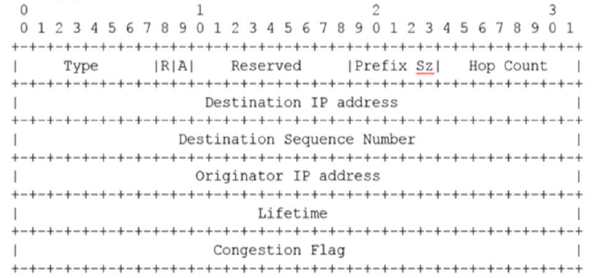
\includegraphics[scale = 0.6]{images/cc-aodv/rrep-header.png}
\caption{New-RREP Packets}.
\label{fig:rrep-header}
\end{figure}

\section{Modifications Made in the Simulator}
For this project, ns-3 network simulator is used and the version of this network simulator is ns-3.35\\
Modifications are made in `src/aodv/model` folder. These are the files where AODV models are implemented.
\subsection{Add Congestion Flag in RREP Packet Header}
\begin{figure}[H]
\centering
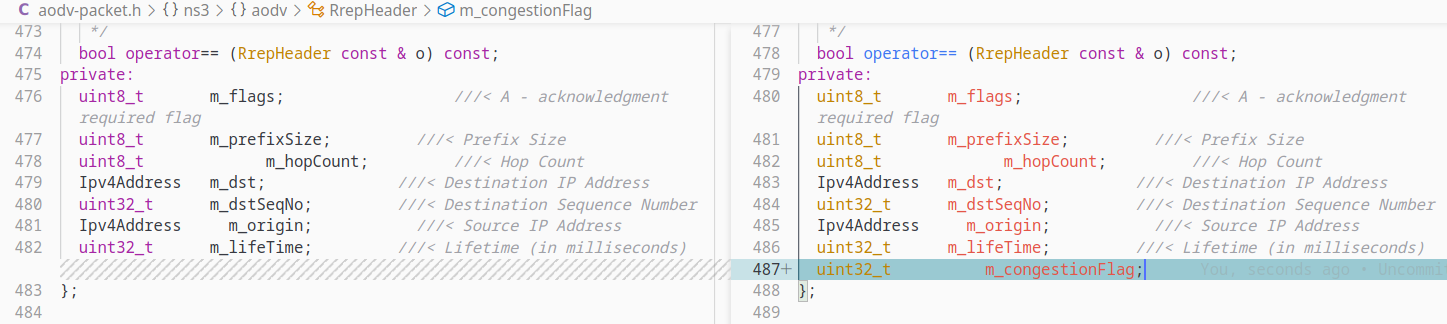
\includegraphics[scale = 0.4]{images/cc-aodv/rrep-01.png}

\end{figure}
\begin{figure}[H]
\centering
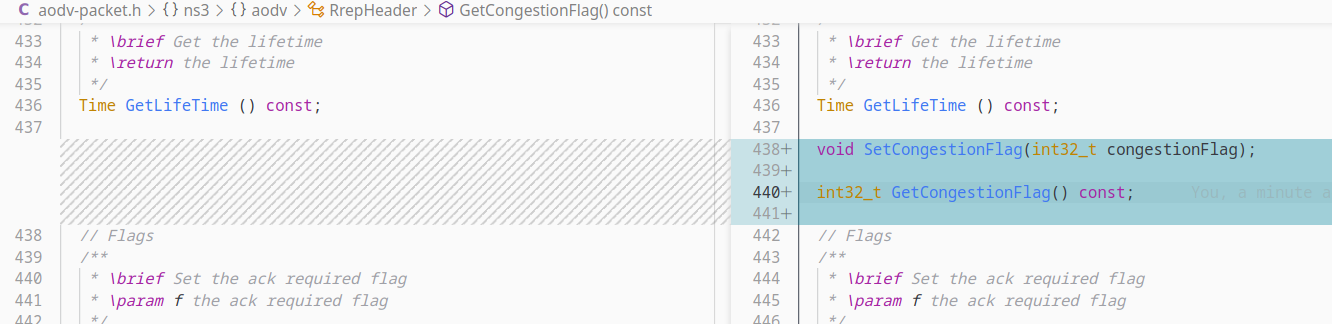
\includegraphics[scale = 0.4]{images/cc-aodv/rrep-02.png}

\end{figure}
\begin{figure}[H]
\centering
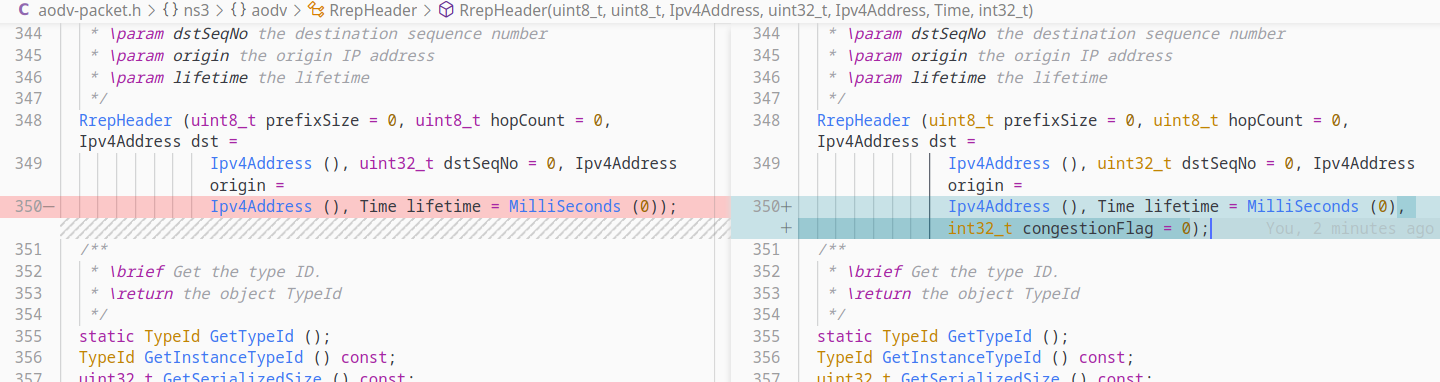
\includegraphics[scale = 0.4]{images/cc-aodv/rrep-03.png}

\end{figure}
\begin{figure}[H]
\centering
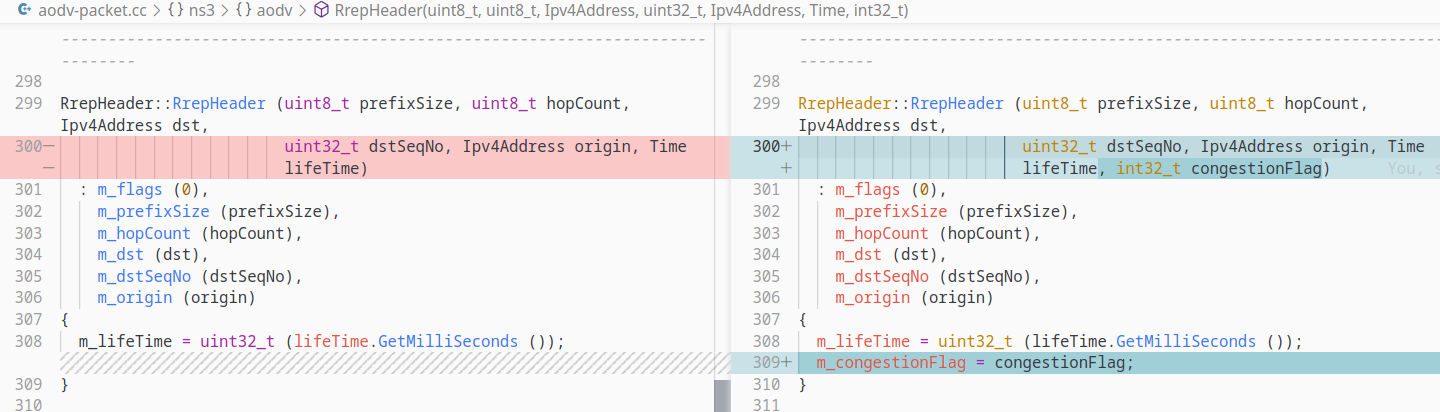
\includegraphics[scale = 0.4]{images/cc-aodv/rrep-04.png}

\end{figure}
\begin{figure}[H]
\centering
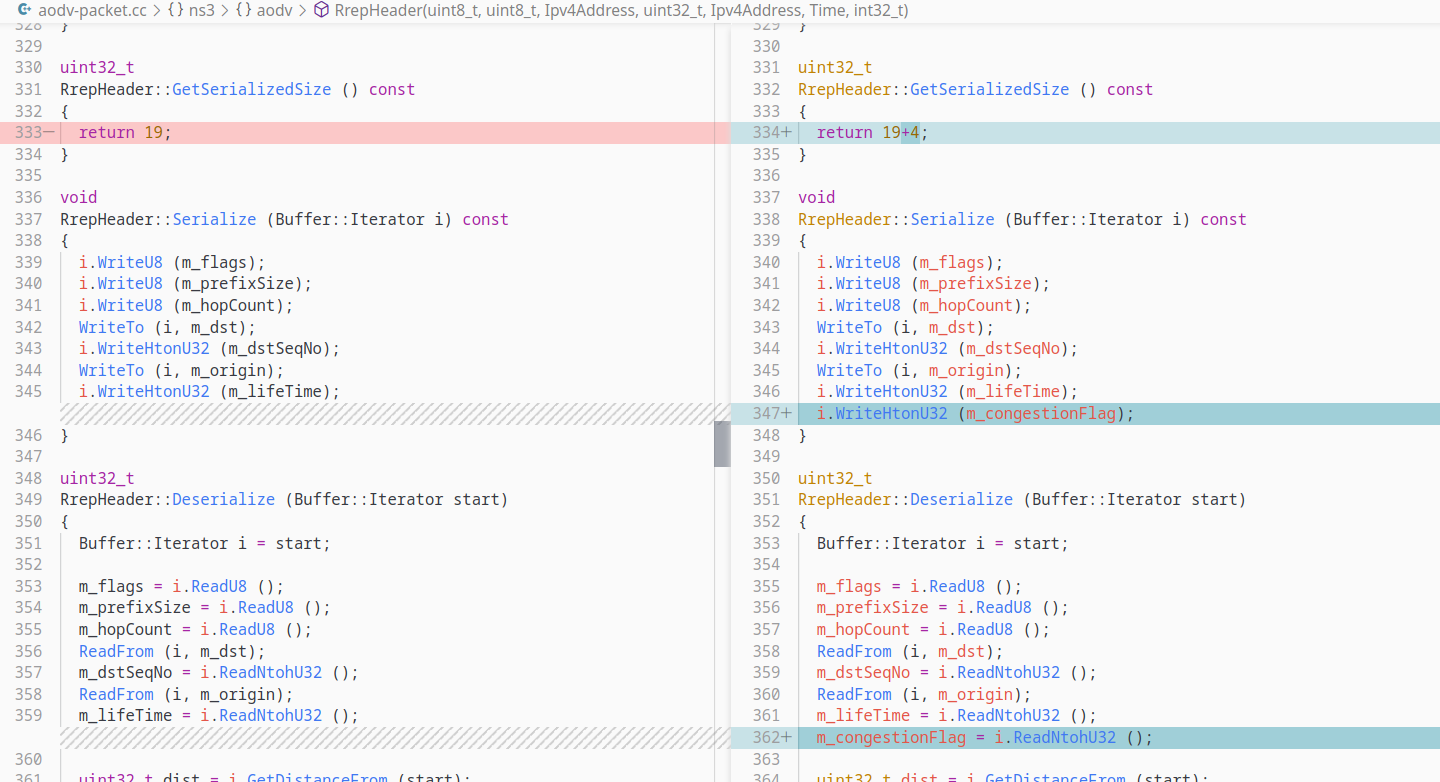
\includegraphics[scale = 0.4]{images/cc-aodv/rrep-05.png}

\end{figure}
\begin{figure}[H]
\centering
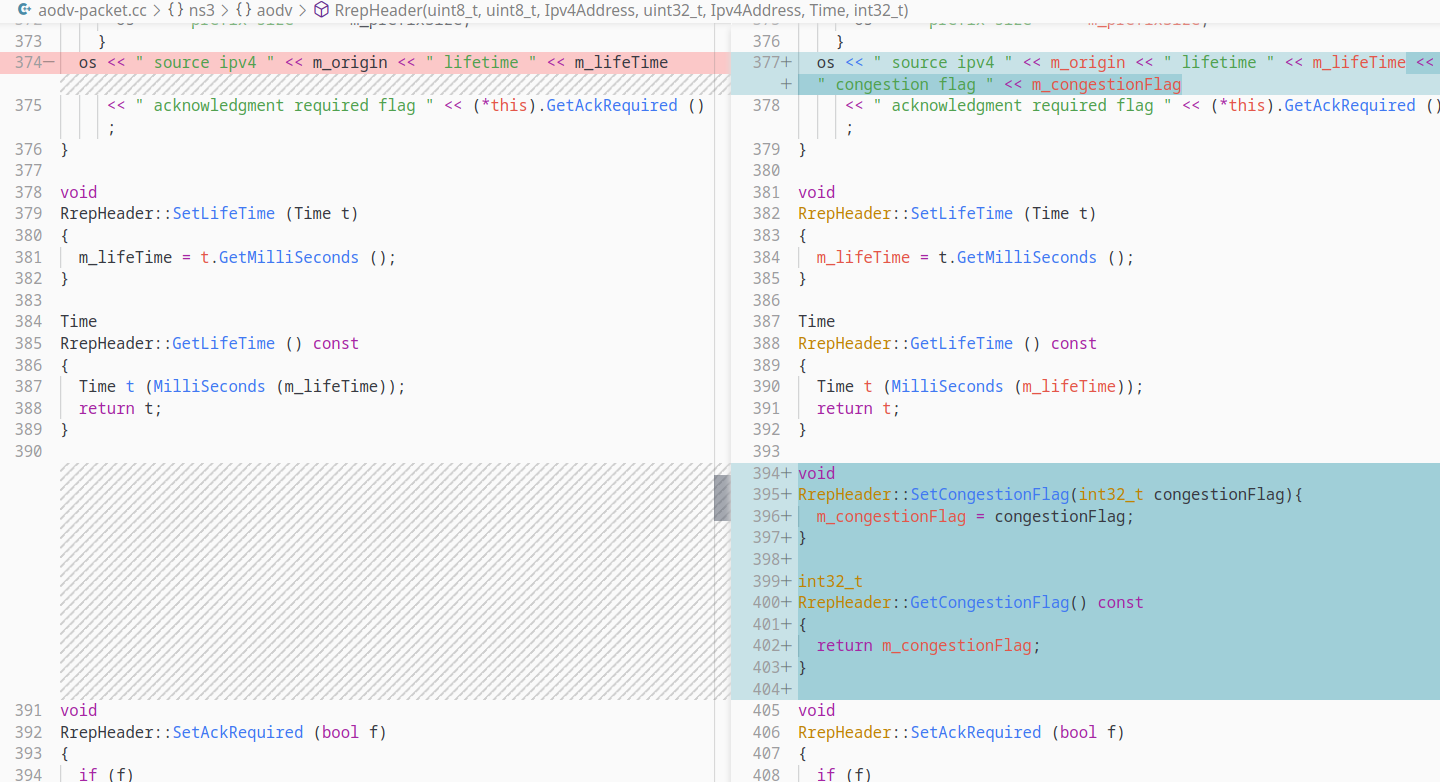
\includegraphics[scale = 0.4]{images/cc-aodv/rrep-06.png}

\end{figure}
\begin{figure}[H]
\centering
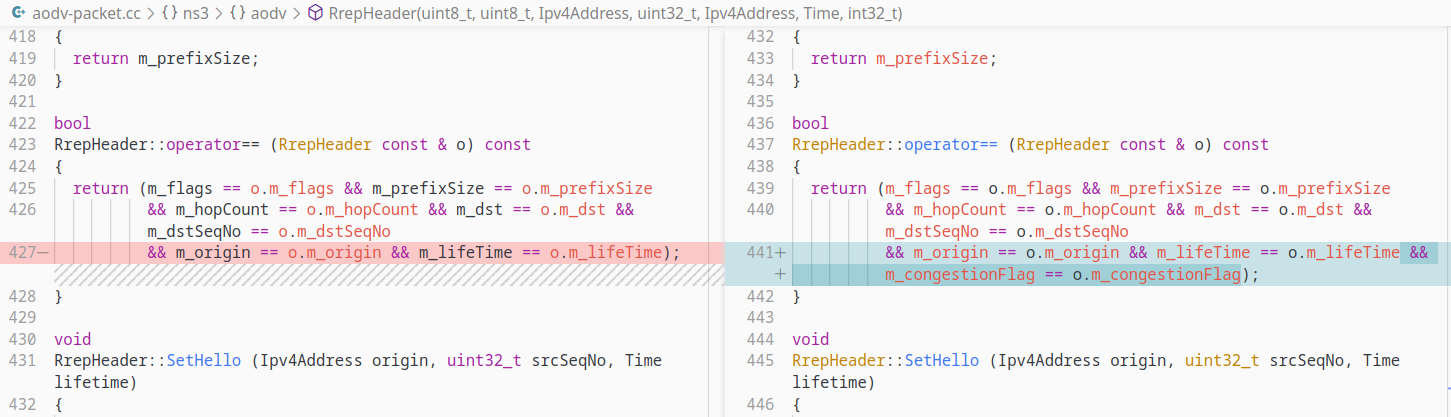
\includegraphics[scale = 0.4]{images/cc-aodv/rrep-07.png}
\end{figure}

\subsection{Congestion Flag in RoutingTableEntry}
\begin{figure}[H]
\centering
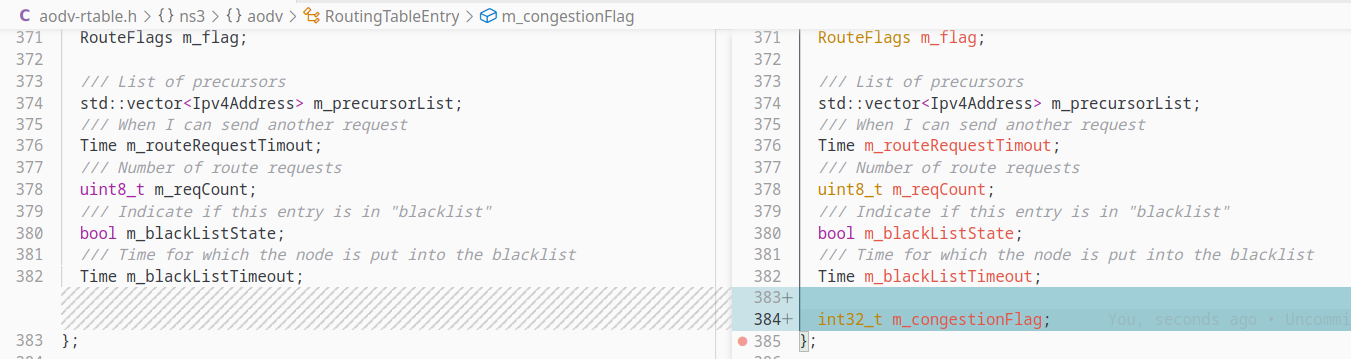
\includegraphics[scale = 0.4]{images/cc-aodv/aodv-01.png}

\end{figure}
\begin{figure}[H]
\centering
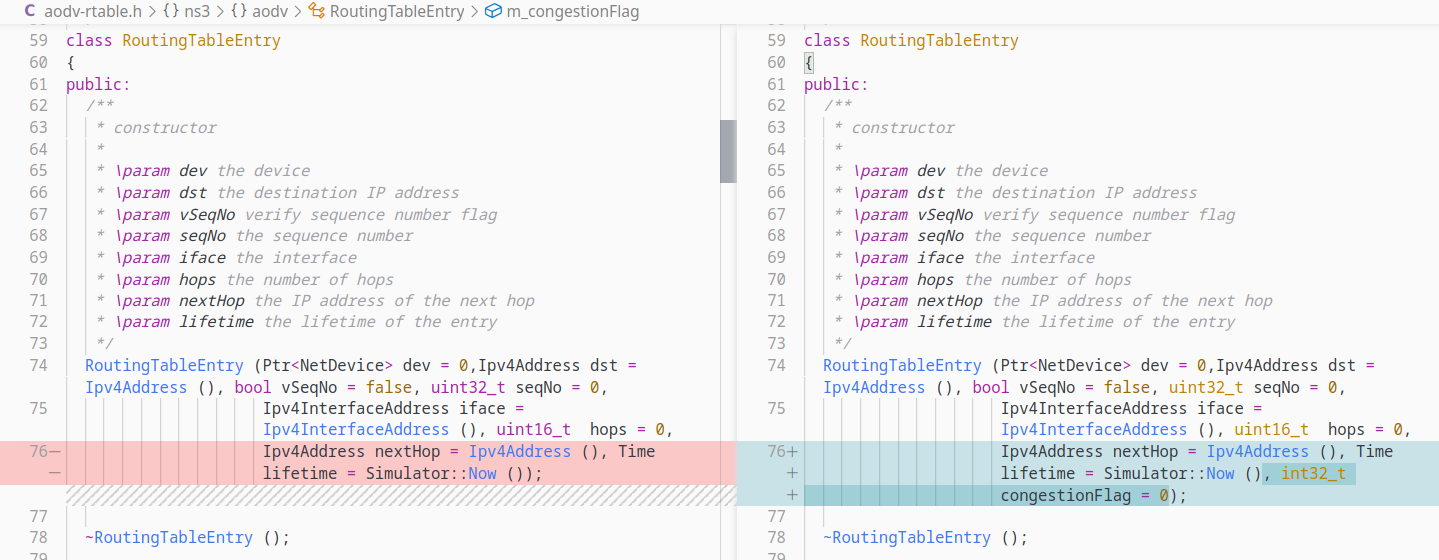
\includegraphics[scale = 0.4]{images/cc-aodv/aodv-02.png}

\end{figure}
\begin{figure}[H]
\centering
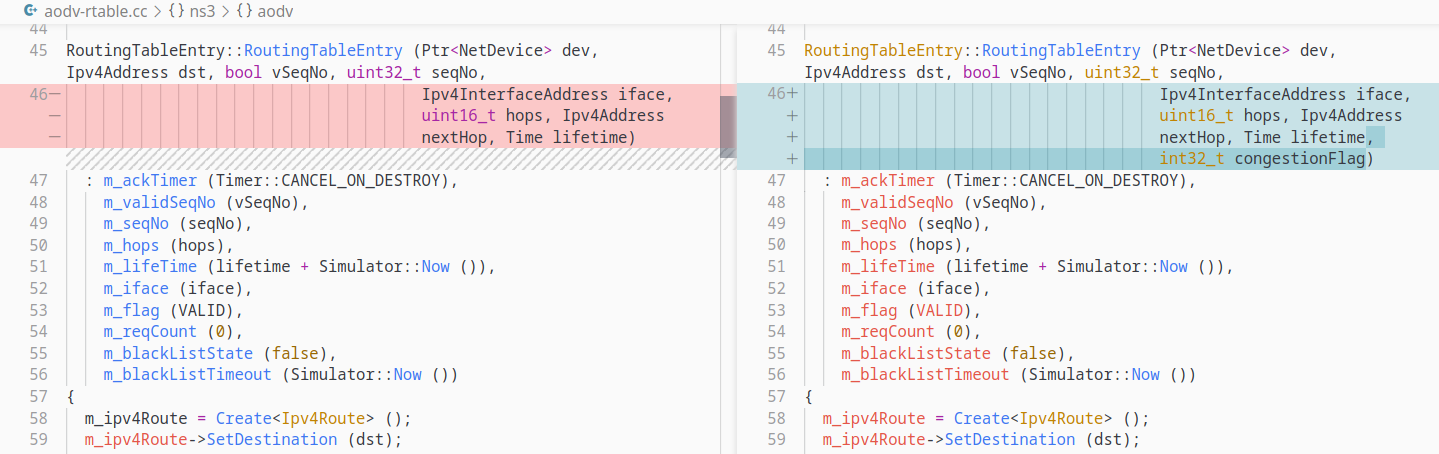
\includegraphics[scale = 0.4]{images/cc-aodv/aodv-03.png}

\end{figure}
\subsection{Add Congestion Counter and Max Count}
\begin{figure}[H]
\centering
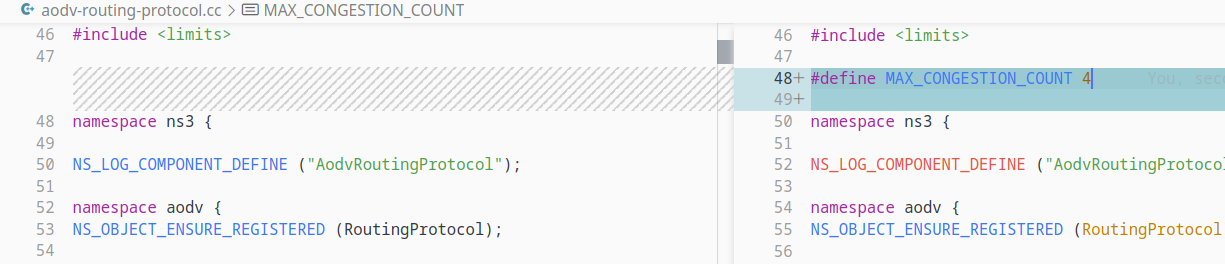
\includegraphics[scale = 0.4]{images/cc-aodv/aodv-04.png}
\end{figure}

\begin{figure}[H]
\centering
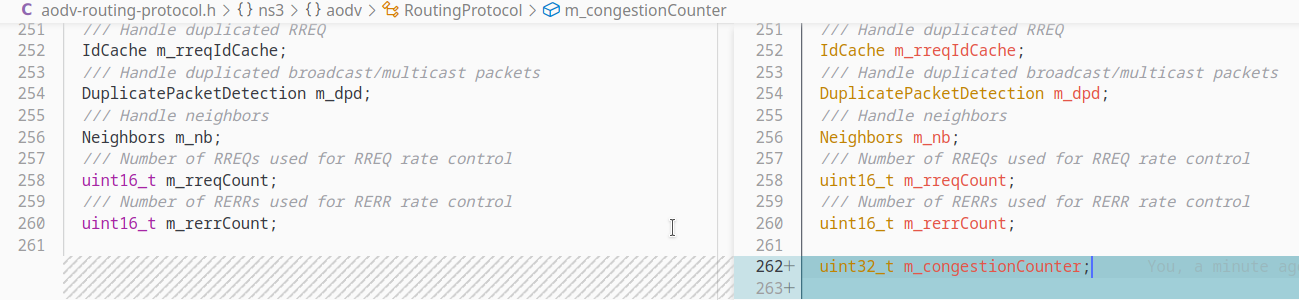
\includegraphics[scale = 0.4]{images/cc-aodv/aodv-05.png}

\end{figure}
\begin{figure}[H]
\centering
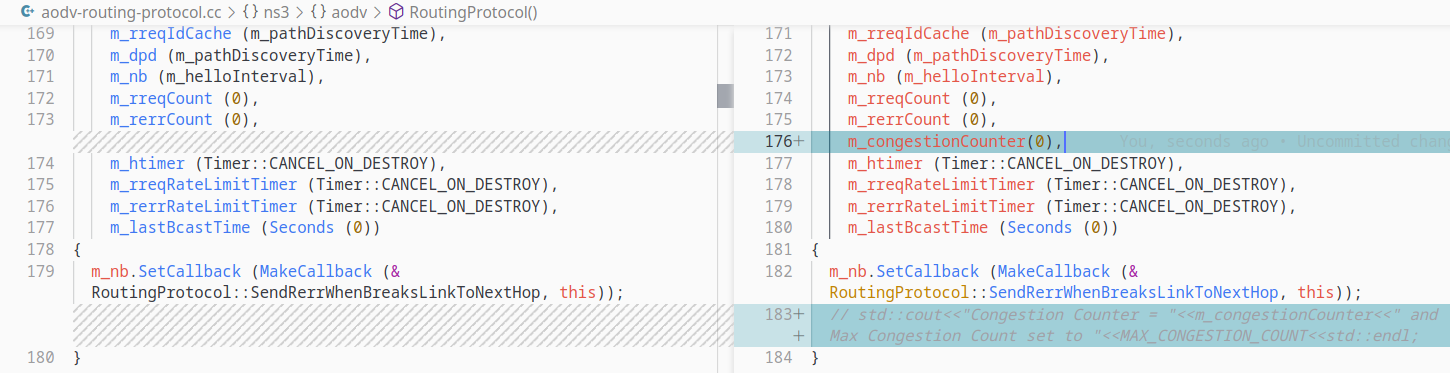
\includegraphics[scale = 0.4]{images/cc-aodv/aodv-06.png}

\end{figure}
\begin{figure}[H]
\centering
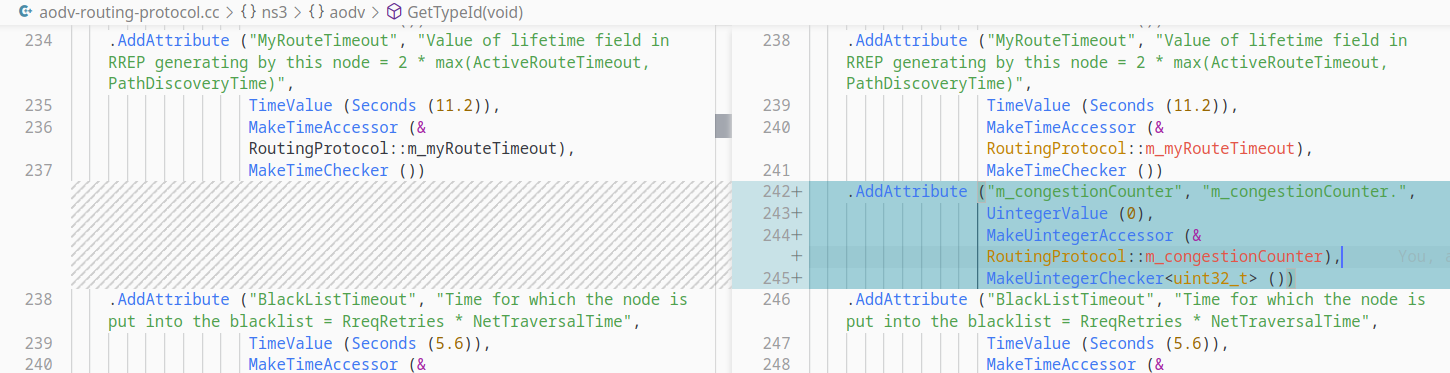
\includegraphics[scale = 0.4]{images/cc-aodv/aodv-07.png}

\end{figure}
\subsection{Drop RREQ Counter Greater than Max Count}
\begin{figure}[H]
\centering
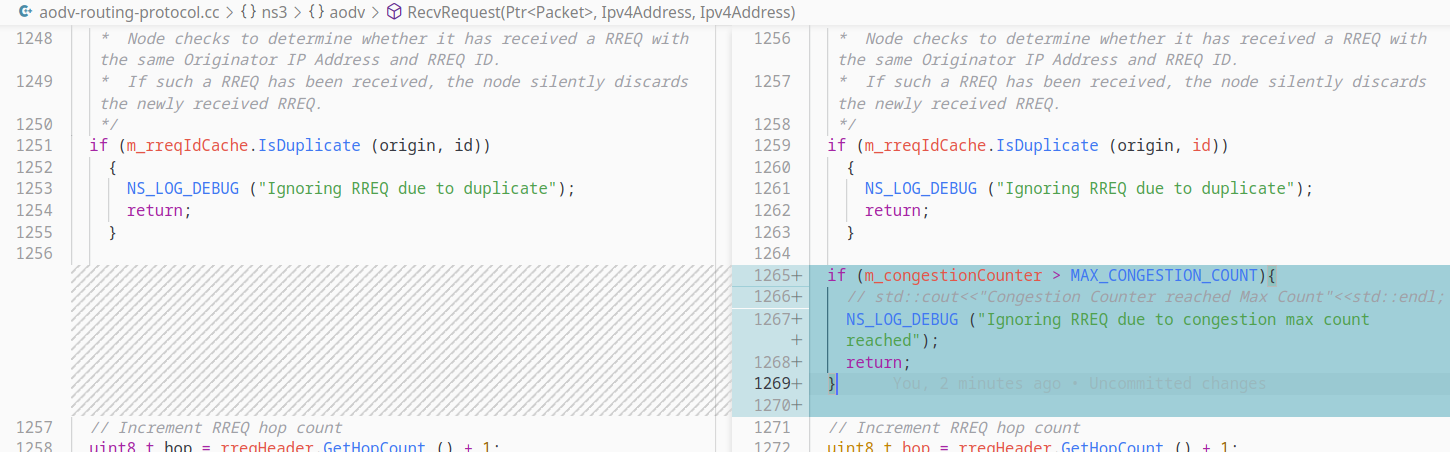
\includegraphics[scale = 0.4]{images/cc-aodv/aodv-08.png}

\end{figure}

\subsection{Counter Increment or Decrement and Flag Operations}
\begin{figure}[H]
\centering
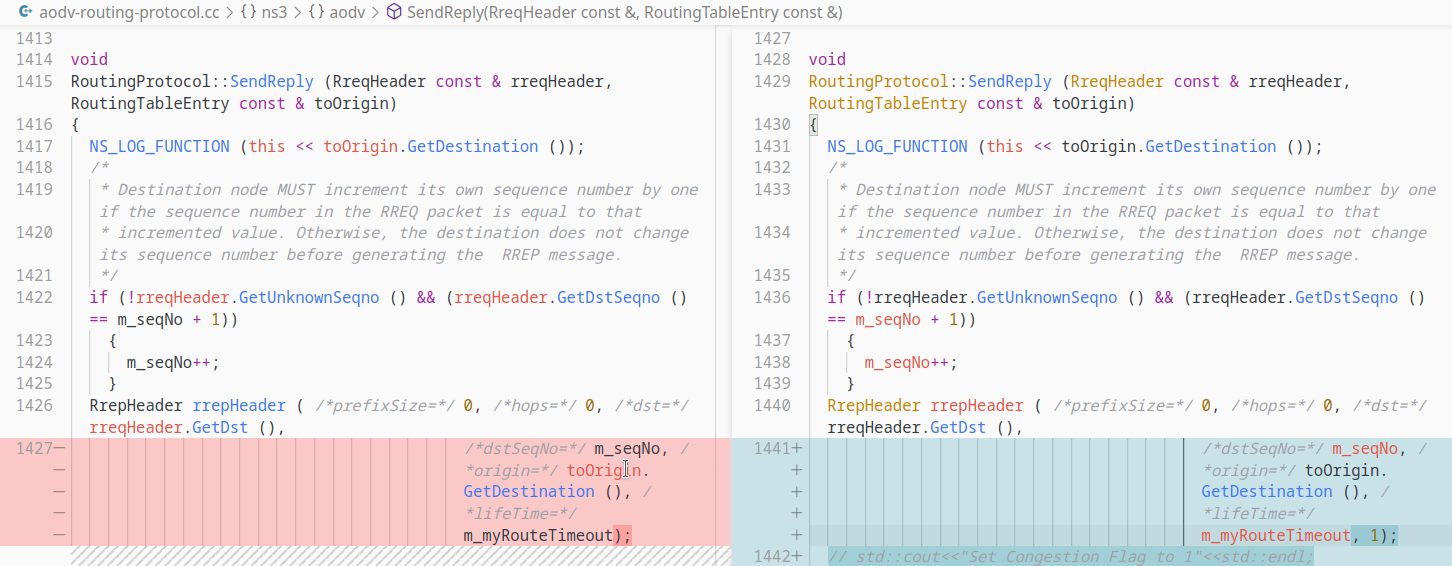
\includegraphics[scale = 0.4]{images/cc-aodv/aodv-09.png}
\end{figure}
\begin{figure}[H]
\centering
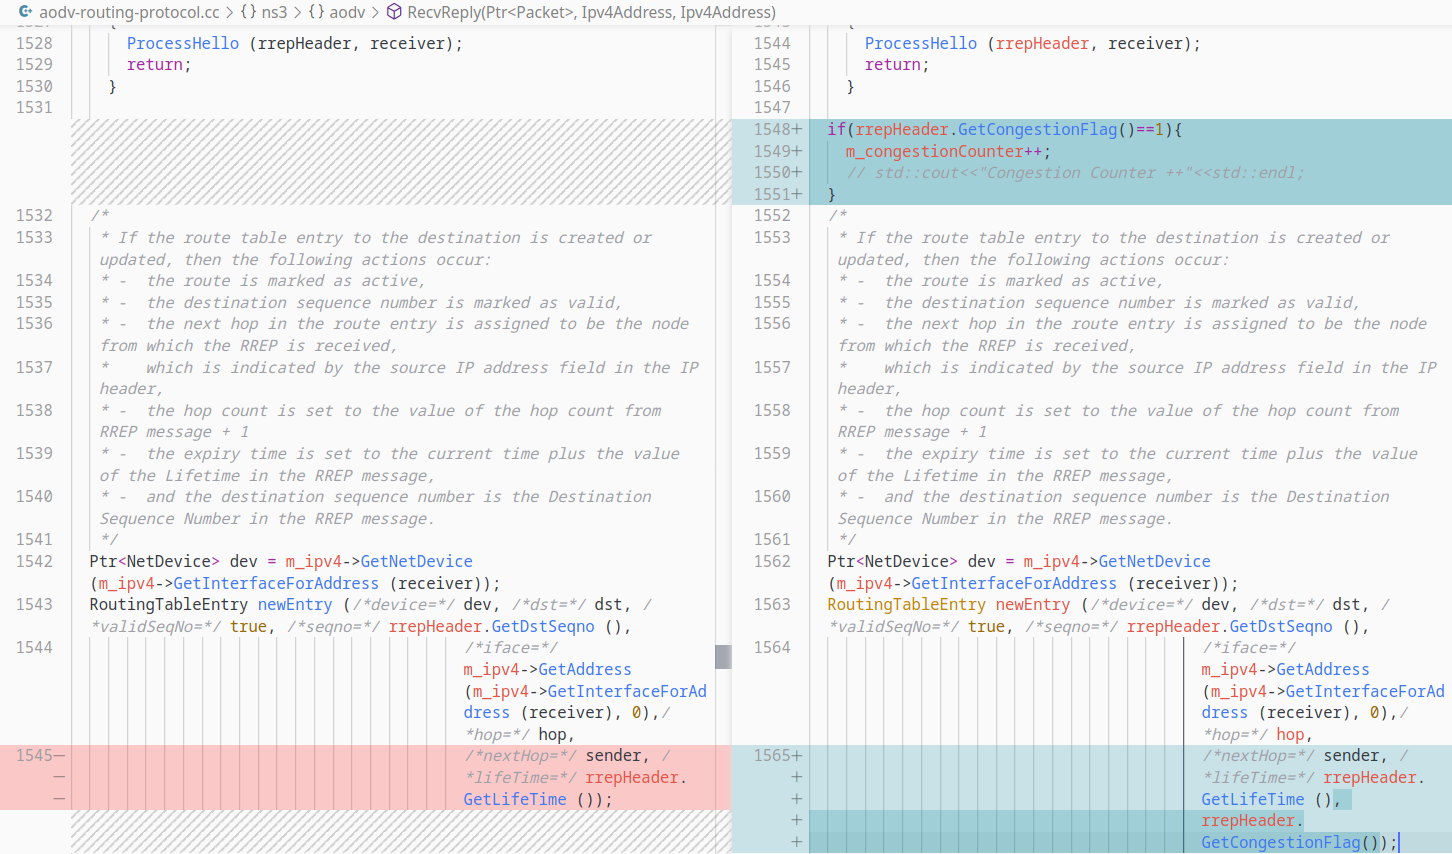
\includegraphics[scale = 0.4]{images/cc-aodv/aodv-10.png}

\end{figure}
\begin{figure}[H]
\centering
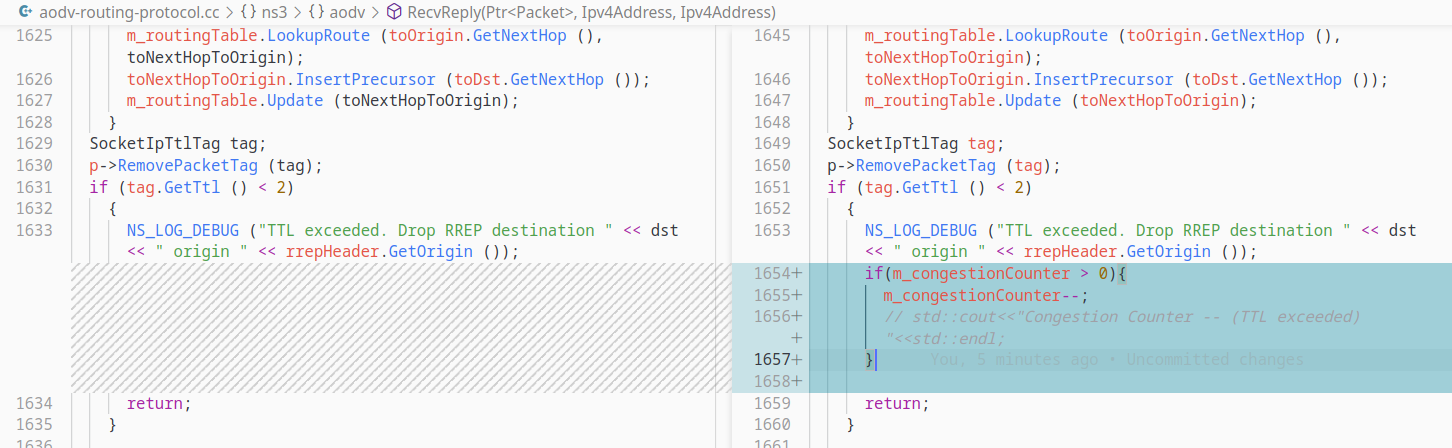
\includegraphics[scale = 0.4]{images/cc-aodv/aodv-11.png}

\end{figure}
\begin{figure}[H]
\centering
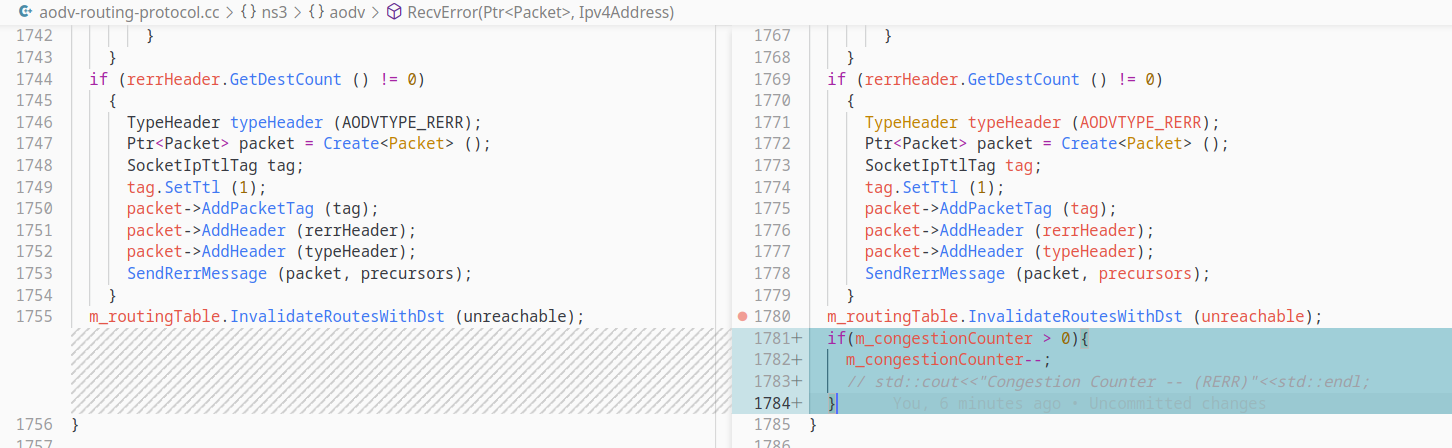
\includegraphics[scale = 0.4]{images/cc-aodv/aodv-12.png}
\end{figure}

\section{Paper Result vs Result of My Task B}
\subsection{Plot Graph}
% 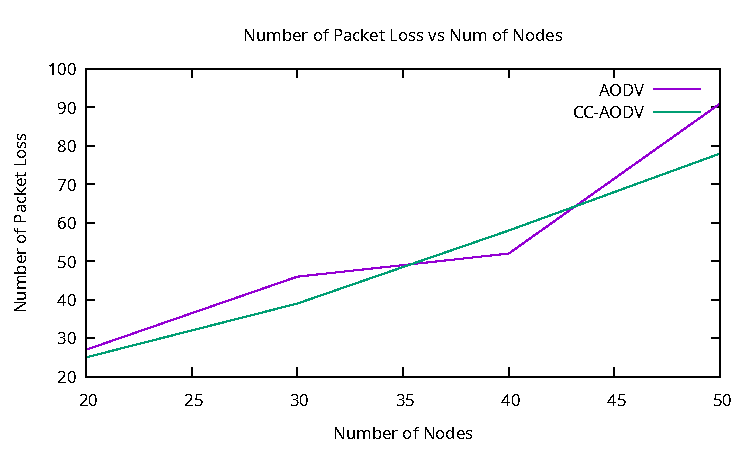
\includepdf[pages=-]{pdfs/TaskB_AODV_Plot.pdf}
\begin{figure}[H]
\centering
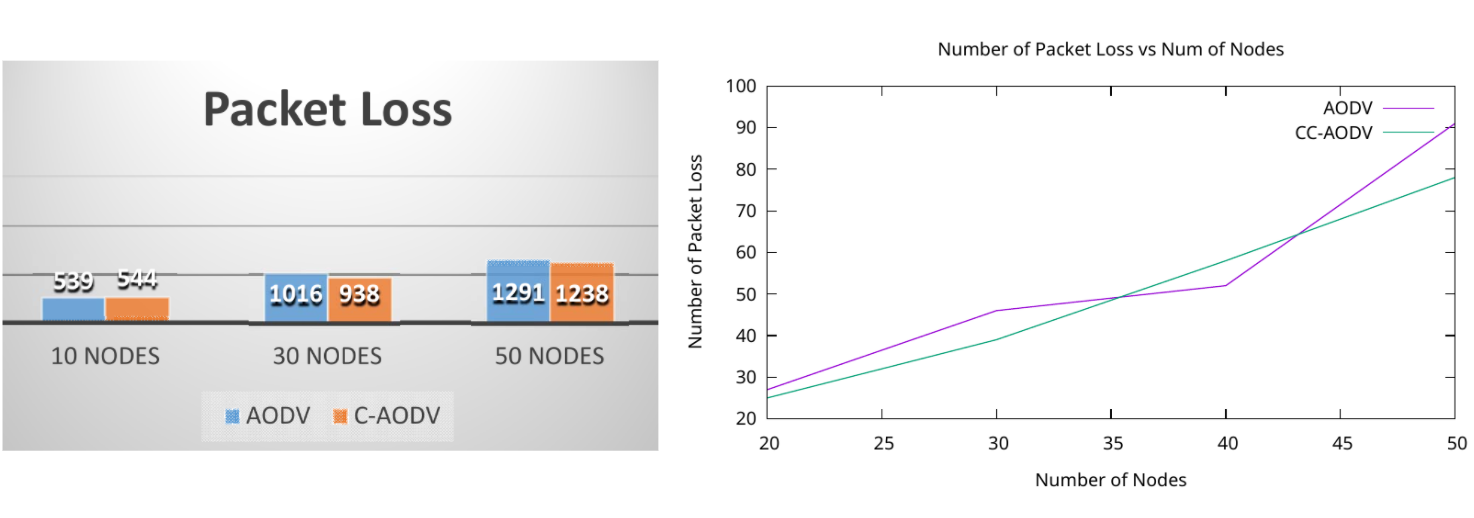
\includegraphics[scale = 0.4]{images/paper/matching-01.png}
\caption{Left: Paper Result, Right: My Result}
\end{figure}

\begin{figure}[H]
\centering
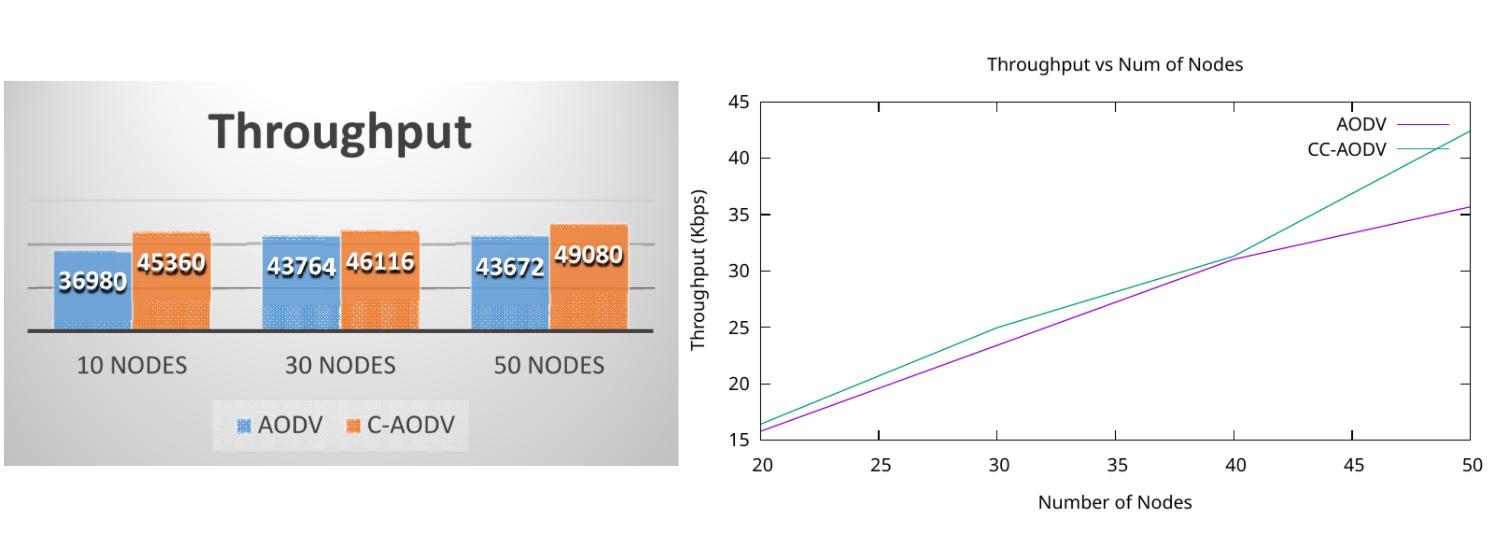
\includegraphics[scale = 0.4]{images/paper/matching-02.png}
\caption{Left: Paper Result, Right: My Result}
\end{figure}

\begin{figure}[H]
\centering
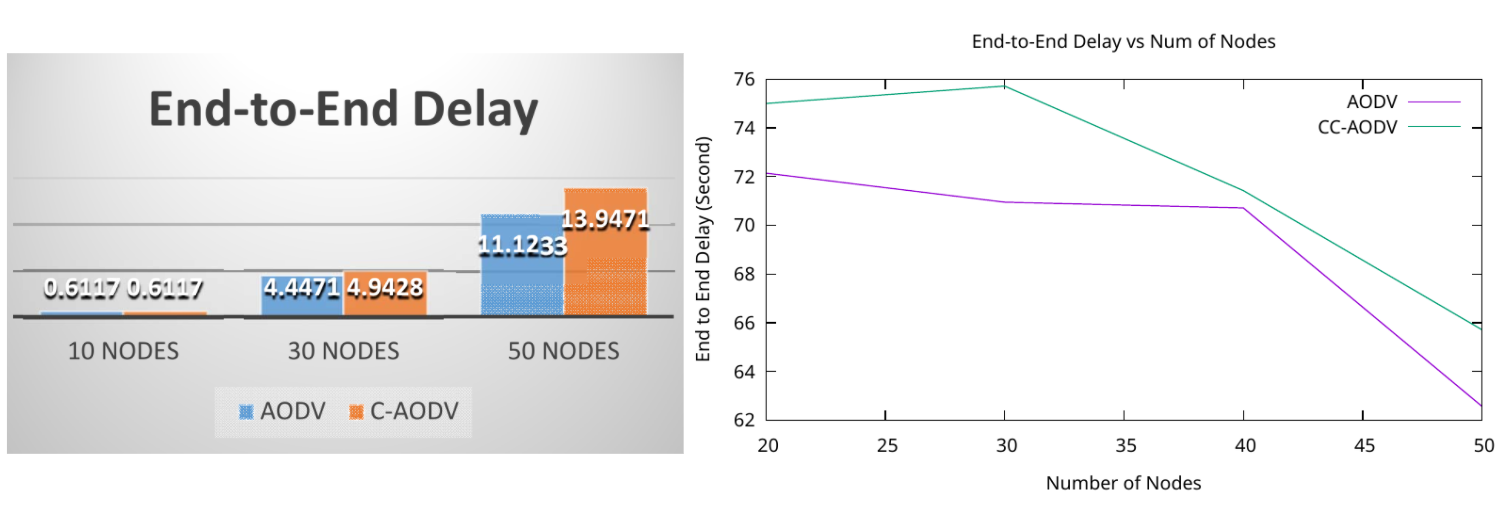
\includegraphics[scale = 0.4]{images/paper/matching-03.png}
\caption{Left: Paper Result, Right: My Result}
\end{figure}

\begin{figure}[H]
\centering
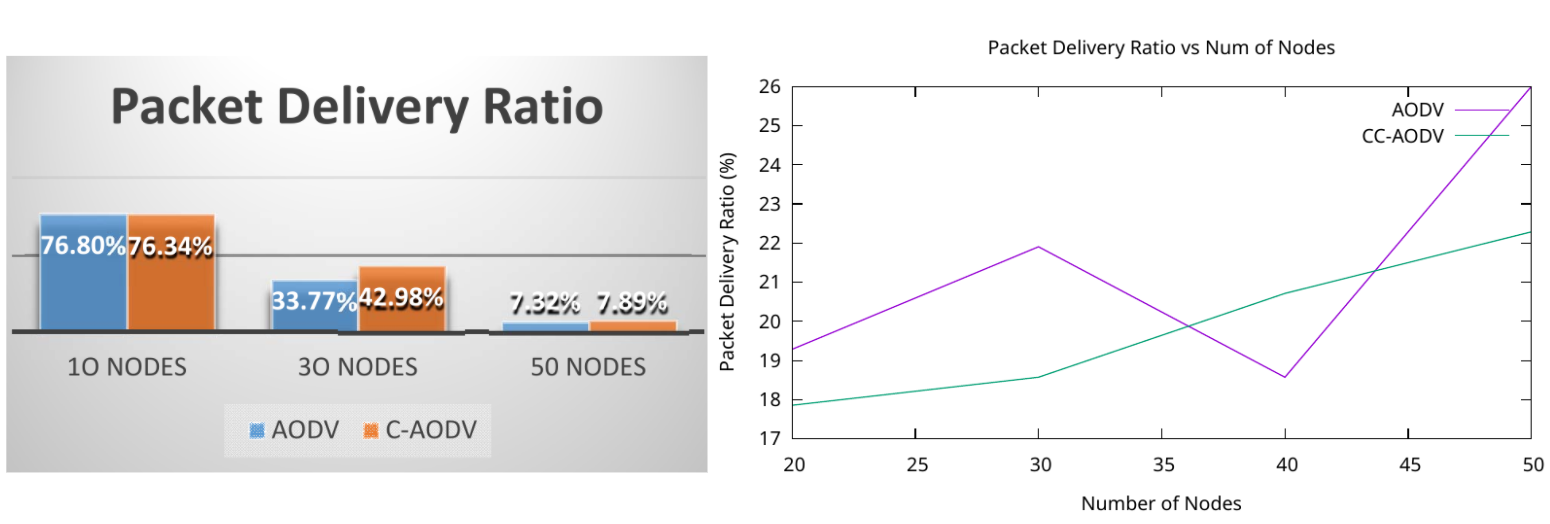
\includegraphics[scale = 0.4]{images/paper/matching-04.png}
\caption{Left: Paper Result, Right: My Result}
\end{figure}
\subsection{My Observation about the Result}
\begin{itemize}
    \item Here we can see that the packet loss graph almost followed the one of the paper. But basic AODV and CC-AODV are nearly same. Not much difference.
    \item We can notice a significant difference in the throughput graph. Throughput is significantly increased.
    \item End to End delay is greater in CC-AODV than basic AODV in both paper simulation and my simulation. In my simulation I have measured the average End to End delay, so the values are not matching with the numeric value range with the paper simulation.
    \item Packet delivery ratio didn't follow the paper very much, but if we look closely, when the number of nodes are near 30, the result are somewhat very near.
    \item In CC-AODV, there is a counter whose value determines whether RREQ packet is sent or dropped. A congestion counter level is used here. I have experimented with some congestion counter level values. I have observed that the congestion counter value influences the packet delivery rate or throughput rate or others. If flow is near 30, and the counter level is set near 4, the result is better than the basic AODV. Increasing the level from 4 to higher will make the result of CC-AODV like the basic AODV. But if the value is lesser than 4, it will not come out with good result. So the tuning is very important here to increase the packet delivery rate or throughput rate or others.
\end{itemize}
\subsection{Minor Improvement Suggestion from my side}
In this paper, they suggested to add a flag in RREP packet header. The flag is only to set true or false, nothing else. But they took a 32 bit flag unnecessarily which is a waste of memory. A boolean variable can be used here. It can be improved.
\section{Results For Task A - Wired Topology}
\subsection{Plot Graph}
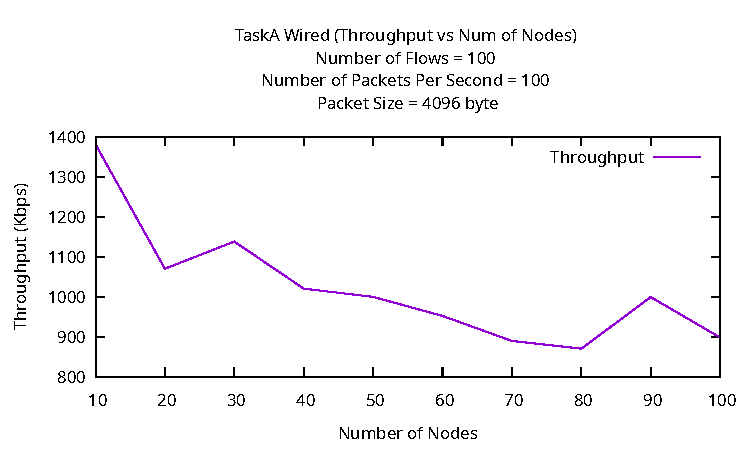
\includepdf[pages=-]{pdfs/TaskA_Wired_Plot.pdf}
\subsection{My Observation about the Result}
\subsubsection{Variation of Number of Nodes}
\begin{itemize}
    \item Increasing the number of nodes causes an increase in the probability that the packet may be dropped while it competes to access the wireless channel at each node to reach its destination.
    \item End to end delay increases with the number of nodes as to go to nodes which is far, it costs time.
    \item Number of nodes increases definitely increases the delivery ratio as number of sink increases. So packet loss ratio decreases.
\end{itemize}
\subsubsection{Variation of Number of Flows}
\begin{itemize}
    \item Increasing number of flows will make race conditions between packets, so throughput may go down. But not always race condition happens.
    \item Increasing number of flows will make go a flow to far away nodes, it will increase the end to end delay.
    \item Number of flows to make many packets drop. So packet delivery ratio will decrease and packet drop ratio will increase.
\end{itemize}
\subsubsection{Variation of Number of Packets Per Second}
\begin{itemize}
    \item The increasing in throughput for larger packets is faster than the increasing for smaller ones. It should increase. But flowmonitor didn't generate good plot this time.
    \item Increasing packets per second should decrease the end to end delay.
    \item Increasing number of packets per second don't results in good graphs because there are many more parameters which are dependent with packets per second. So packet delivery ratio, packet drop ratio didn't well simulated here.
\end{itemize}
\section{Results For Task A - Wireless Low Rate (Static)}
\subsection{Plot Graph}
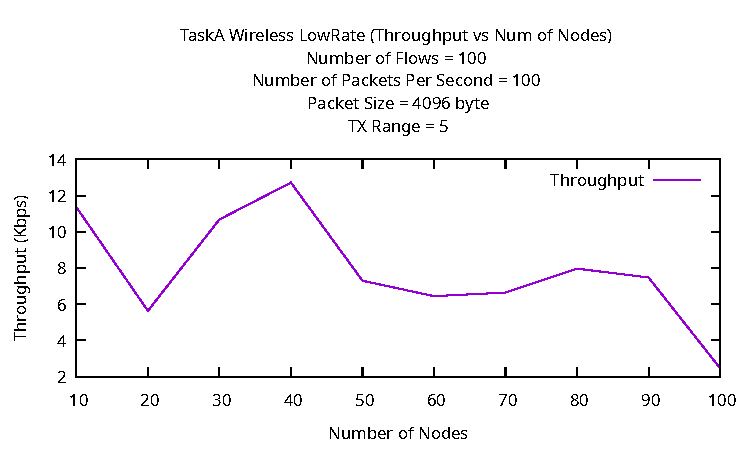
\includepdf[pages=-]{pdfs/TaskA_Wireless_LowRate_Plot.pdf}
\subsection{My Observation about the Result}
\subsubsection{Variation of Number of Nodes}
\begin{itemize}
    \item Increasing the number of nodes causes an increase in the probability that the packet may be dropped while it competes to access the wireless channel at each node to reach its destination.
    \item End to end delay should be less with the increasing number of nodes. But this is here low rate, so may not behave well due to low rate. Delay may be increased.
    \item If it were wired, packet delivery ratio would be high with the number of nodes. But here in low rate, packet may not be delivered due to low rate. Packet loss ratio is vice versa.
\end{itemize}

\subsubsection{Variation of Number of Flows}
\begin{itemize}
    \item Increasing number of flows make many packets to drop, so throughput goes down.
    \item End to end delay increases with the number of flows.
    \item Packet delivery ratio should increase with the number of flows. But due to low rate, it may misbehave.
\end{itemize}
\subsubsection{Variation of Number of Packets Per Second}
\begin{itemize}
    \item Throughput increases with the number of packets per second.
    \item End to end delay decreases with the number of packets per second.
    \item Packet delivery ratio increases with the number of packets per second. Loss ratio is vice versa.
\end{itemize}
\subsubsection{Variation of Tx Range}
\begin{itemize}
    \item Increasing TX range makes a packet to travel more distance. So throughput increases, packet delivery ratio increases, packet drop ratio decreases. 
    \item End to end delay increases as the packet can travel more distance.
\end{itemize}

\section{Conclusion}
This project introduced us with NS-3. It is one of the leading network simulating tool. It was difficult to work with for the first time, but with the co-operations of peers and supervisors, NS3 experience has gone well. Hope to work on computer networks in future.\\
Source codes of this project is available in my Github Repository. \url{https://github.com/kawshikbuet17/Congestion-Control-AODV}


\begin{thebibliography}{9}
\bibitem{texbook}
CC-ADOV: An effective multiple paths congestion control AODV\\
Yefa Mai, Fernando Molina Rodriguez, Nan Wang, \url{https://ieeexplore.ieee.org/document/8301758}
\end{thebibliography}
\end{document}